\subsection{Specification of Boundary Conditions for the Input Geometry}
\label{sec: GeomCreation}

\begin{figure}
\centering
  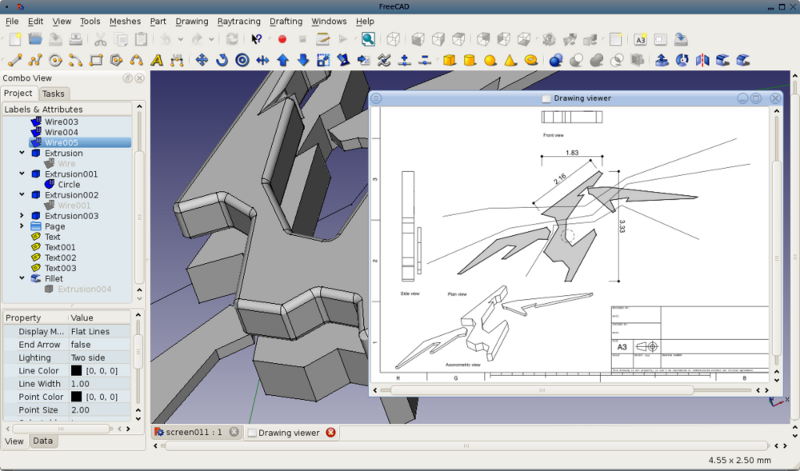
\includegraphics[scale=0.75]{Pictures/CADToVoxel/FreeCAD.png}
\caption{The FreeCAD workbench. FreeCAD is an open-source CAD modeling software, and is the primary CAD tool used in this project.\cite{FreeCAD}}
\label{fig: freeCAD}
\end{figure}

As pointed out in the \ref{CADbackg}, STEP and IGES files can store color information for each face. This is the attribute that is used to specify the identity of the face. When analysing a structural problem, a designer typically needs to provide information on four parameters:

\begin{itemize}
	\item \textbf{Fixture faces}: These faces of the geometry are meant to be fixed in space, and undergo zero displacement. These faces are colored absolute red, i.e. if the color space of red ranges in {$[0, 255]$}, then the face is assigned the extremum $255$. The blue and green color components are set to $0$. Thus, the color array is set to $(255, 0, 0)$
	\item \textbf{Load faces and load value}: These faces bear the forces acting on the body. Loads are three-dimensional, and can take both positive and negative values depending on their direction. To accommodate all possibilities, each color component (i.e. red, blue and green) is assigned a direction ($x$, $y$, and $z$). The range $(0, 255)$ is split in two: $(0, 127]$ representing the negative force range and $[128, 255)$ representing the positive force range. The color is then offset by $-127$. 

Of course, force values may also lie outside the offset color range, i.e $(-\infty, -127] \cup [128, \infty)$. The user then needs to scale the required force to fit in the color range, and provide a scaling factor as an input.

For example, to assign a force value of $(-200.5, 172.0, -10.75)$:

\begin{table}[h!]
	\begin{center}
		\caption{Fitting a force value to a color}
		\label{LoadFaceExample}
		\begin{tabular}{cccc}
			\toprule
			{\small Original vector} & {\small Scaling factor} & {\small Modified vector} & {\small Final color}\\
			\midrule
			$-200.5$ & $0.628428928$ & $-126$ & $1$\\
			$172.0$  & $0.628428928$ & $108$  & $235$\\
			$-10.75$ & $0.628428928$ & $-7$   & $120$\\
			\bottomrule
		\end{tabular}
	\end{center}
\end{table}
	\item \textbf{Non-changing faces}: Sometimes, certain parts of the geometry cannot accommodate changes. This could be for several reasons, for example, due to compatibility issues with other components. These faces are marked with absolute green, i.e. $(0, 255, 0)$.
	\item \textbf{The original geometry}: This refers to the geometry that needs to be optimised. These faces are simply colored absolute black, i.e. $(0, 0, 0)$.
\end{itemize}

The user must save the CAD file in both STEP and IGES formats. This is necessary due to some issues with the face extraction process in OpenCascade - the IGES format allows for proper face extraction, but color detection works only for the STEP format. Also, the files should be saved in the same directory, and have the same name.
